\documentclass[../TinyBot.tex]{subfiles}
\begin{document}

\section{Wiring} \label{wiring}
If you just want to see the wiring schematic, see Figure \ref{fig:schematic-hbridge}. Continue reading for an explanation of the L293D H-Bridge and of the circuit. 

\bigskip

Before starting construction on any project, it is always a good idea to wire up the circuit on a flat breadboard and arduino; as it is far easier to build the circuit on its own before putting together all the parts. \\

Datasheets hold a lot of useful information about microchips, the data sheet for the L293D H-Bridge can can be found online (linked \href{https://www.altronics.com.au/p/z2900-l293d-motor-drive-ic/}{here}).

\begin{figure}[h]
    \centering
     \begin{subfigure}[b]{0.5\textwidth}
         \centering
         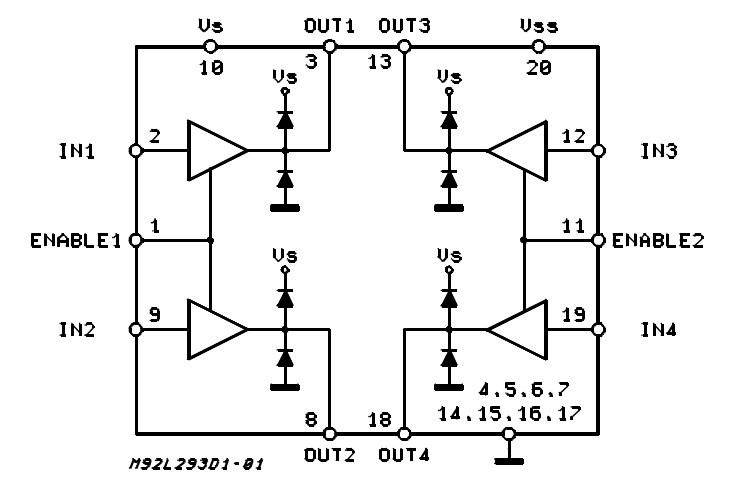
\includegraphics[width=\textwidth]{L293D-block-diagram.jpg}
         \caption{Block Diagram for 20 Pin Chip}
         \label{fig:l293d-block-diagram}
     \end{subfigure}
     \hfill
     \begin{subfigure}[b]{0.3\textwidth}
         \centering
         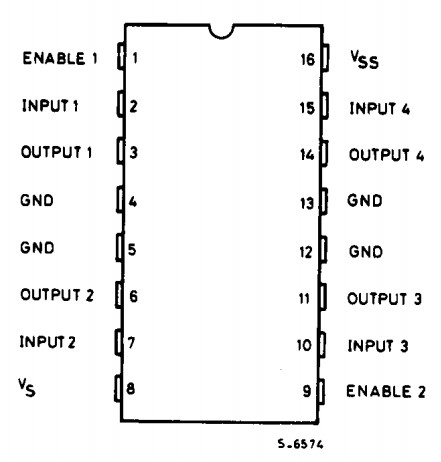
\includegraphics[width=\textwidth]{L293D-pinout.jpg}
         \caption{Pinout of 16 Pin Chip}
         \label{fig:l293d-pinout}
     \end{subfigure}
     \hfill
        \caption{Diagrams from the L293D datasheet}
        \label{fig:l293d}
\end{figure}

Block diagrams such as in Figure \ref{fig:l293d-block-diagram} can be quite confusing to read; there's a lot of symbols that you may or may not know. 

The hollow circles along the outside rectangle of the block diagram in Figure \ref{fig:l293d-block-diagram} represent the pin outs on the microchip, they can be matched up with labelled pins in Figure \ref{fig:l293d-pinout}. There is also a 20 pin variant of this H-bridge, which is why some of the pin labels on the block diagram are greater than 16.\\

The hollow triangles in the block diagram are buffers to drive the MOSFET (depicted the bold black triangle and lines, which are the "switches" in this H-Bridge). Basically, setting \lstinline[]!IN1=HIGH! when \lstinline[]!ENABLE1=HIGH! will close the switch and provide power to \lstinline[]!OUT1!. 

Using the buffer allows a low voltage signal, from the digital ports on the Arduino, to close the switch and allow the higher voltage from \lstinline[]!ENABLE1! to flow through to the motor. If \lstinline[]!ENABLE! has no power, then the motor will not turn; the voltage provided from the digital pins is not sufficient to drive the motor.  This is why in Figure \ref{fig:schematic-hbridge} you'll notice that all 4 \lstinline[]!ENABLE! pins are all linked and permanently set to 9V (\lstinline[]!HIGH!) \\


A MOSFET (mentioned above) is an advanced digital component, not discussed in University till about 3rd year engineering units. They are quite complicated components, though can be effectively summed up as an electrically controlled switch. Providing the right signal to the MOSFET will allow current to flow in much the same manner as pressing a push buttons allows current to flow. This information about MOSFETs is included for completeness, and to satisfy any curiosity. It is not important to understand MOSFETs at this level, though if you are curious the internet has many resources available for learning about elecitrical components in depth. \\

\begin{center}
    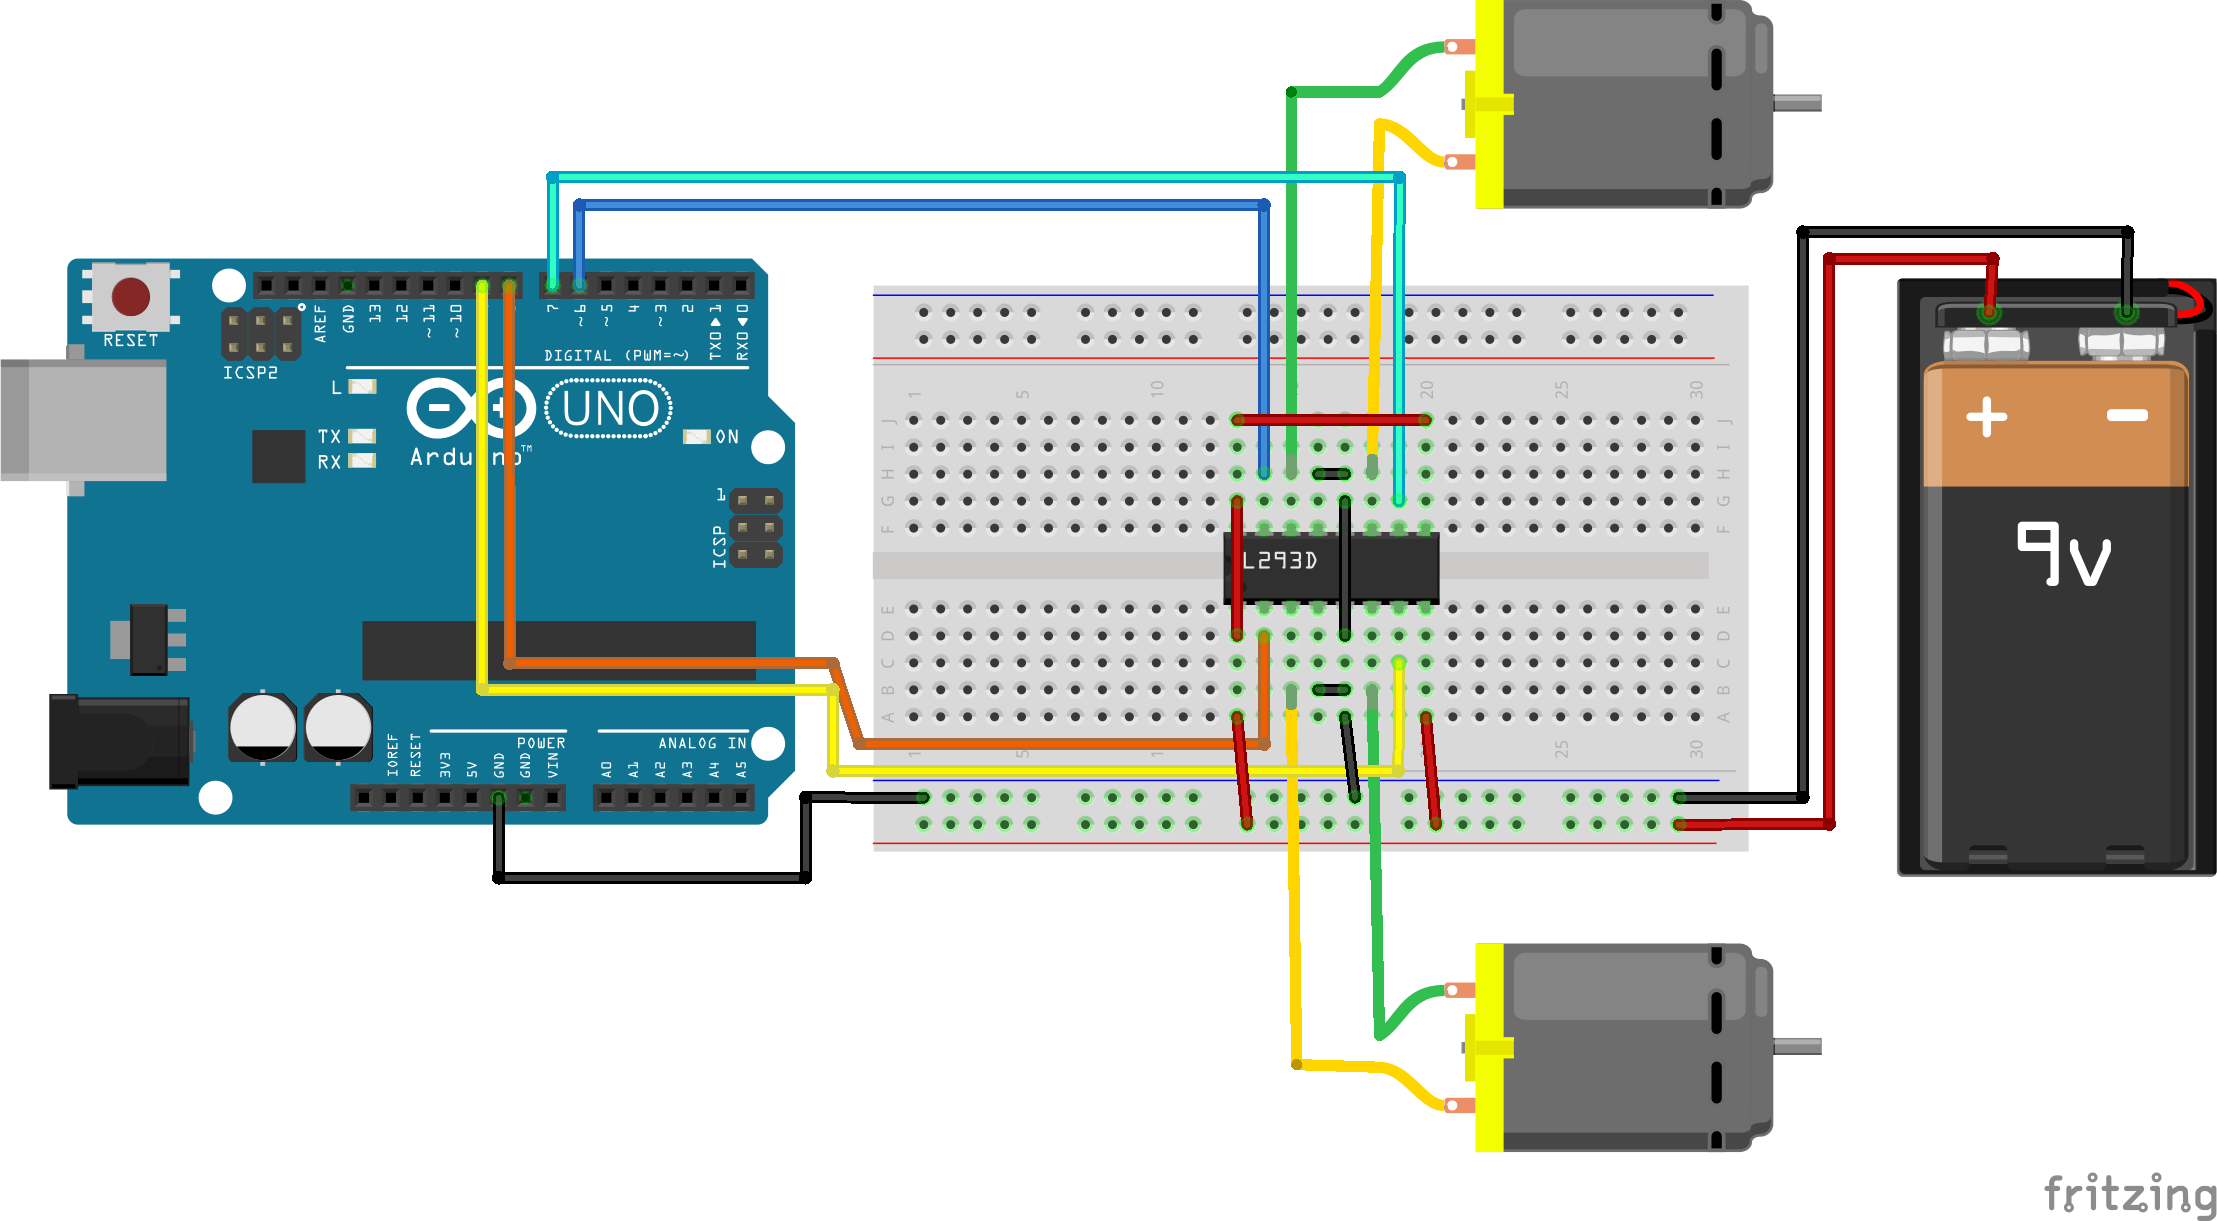
\includegraphics[width=\textwidth]{Hbridge_bb.png}
    \captionof{figure}{Wiring Schematic for H-Bridge}
    \label{fig:schematic-hbridge}
\end{center}

Make sure to check which wire is the positive wire on the motor you have, it should be written on the back plate of the motor. Plugging the motor in backwards will not break anything, the motor will just spin backwards. 
It is mainly important to ensure that the motors spin in the same direction. 



\end{document}